\documentclass{article}
\usepackage{amsmath}
\usepackage{anyfontsize}
\usepackage{colortbl}
\usepackage{geometry}
\usepackage{graphicx}
\usepackage{hhline}
\usepackage{hyperref}
\usepackage{ragged2e}
\usepackage{tabularx}
\usepackage{titlesec}
\usepackage{tcolorbox}
\usepackage{xcolor}
\usepackage{amssymb}
\usepackage{fontawesome}
\usepackage{soul}
\usepackage{float}
\usepackage{fancyhdr}
\usepackage{tocloft}
\usepackage{pifont}
\usepackage{listings}
\usepackage{xcolor}
\usepackage{url}

\lstset{ 
  language=C,
  basicstyle=\ttfamily,
  keywordstyle=\color{blue!90!black},
  stringstyle=\color{red!80!black},
  commentstyle=\color{green!60!black},
  morecomment=[l][\color{purple!80!black}]{\#},
  frame=single,
  numbers=left,
  numberstyle=\tiny\color{gray},
  backgroundcolor=\color{gray!5},
  showstringspaces=false,
  breaklines=true,
  breakatwhitespace=true
}

% Header setup
\pagestyle{fancy}
\fancyhf{}
\fancyhead[L]{\leftmark}  % Section title on the left
\fancyhead[R]{\thepage}   % Page number on the right

\definecolor{PrussianBlue}{RGB}{0,43,73}
\definecolor{LightBlue}{RGB}{230,255,255}

\begin{document}

\begin{titlepage}
    \centering
    
\includegraphics[width=0.75\textwidth]{img/logo.png}\par
    \vspace{0.5cm}
    {\scshape\Huge FreeRTOS: Rate Monotonic Scheduling \par}
    \vspace{1cm}
    {\scshape\LARGE Computer Architectures and Operating Systems Project (Track 1.2: HaclOSsim) \par}
    \vspace{2cm}
    \begin{tabularx}{\textwidth}{Xr}
        \begin{minipage}[t]{0.45\textwidth}
            \raggedright
            {\Large Authors: \\ Merico Michele \\ Marino Alberto \\ Maniero Edoardo \\ Seidita Nicola \par}
        \end{minipage} &
        \begin{minipage}[t]{0.45\textwidth}
            \raggedleft
            {\Large  \par}
        \end{minipage}
    \end{tabularx}
    \vfill
    \hrule height 0.5pt
    \vspace{0.5cm}
    {\Large Academic Year 2023/2024 \par}
\end{titlepage}

% Include chapter files
\section{Introduction}
In this project, the FreeRTOS scheduling mechanism will be analysed and modifications will be made to implement Rate Monotonic (RM) Scheduling. Subsequently, the performance of the original FreeRTOS scheduling will be compared with that of RM Scheduling, evaluating the efficiency in managing task priorities and execution times.

\subsection{What is FreeRTOS}
FreeRTOS is an independent, small, simple real-time operating system kernel being released freely for the use of microcontroller-based applications. It was developed by Richard Barry in the year 2003; this is a simple, strongly typed, and very light kernel that supports multitasking applications in need of accurate timing. Its features include high portability, unrestricted use of asserts, scalability and supported microcontroller architectures that makes it to be largely used in automotive, industrial automation, and consumer electronics industries. Thus, it can be employed in devices with a limited amount of resources while still supporting intricate functionalities. It is now used by a vast number of people and well-documented which makes FreeRTOS a reliable solution for real-time systems used in the field of embedded systems.

\subsection{FreeRTOS Scheduling}
The system scheduler employed in FreeRTOS is preemptive priority based whereby a set of tasks with different priorities can effectively be dealt with. The following scheduler ensures that the maximum priority task, that is, the one that is prepared to run is every given CPU time. If, however, there are several tasks with the same priority level, FreeRTOS will allow them to be serviced in a circular basis, to give each of them approximately equal time on the processor. 

\noindent To enhance multitasking, FreeRTOS has other attributes that enable the developers to develop more than one task at a time. Every task under FreeRTOS runs in the form of a thread with stack and the kernel SW is responsible for task swapping. Context switching is a type of operating system scheduling mechanism in which the operating system saves the state of the presently executing task and restores the state of the task set to be executed next. This makes it possible for each of the tasks to continue with the execution from where it was interrupted. 

\noindent FreeRTOS also provides features like semaphores, mutexes and event group which assist in controlling the execution of tasks and controlling access to the resources. Race conditions are thus avoided, and it becomes certain that one task will not intrude with the other when both are accessing vital parts of the code or data. Also, FreeRTOS provides mechanisms for tasks’ interaction through message passing using message queues and stream buffers. 

\noindent In conclusion, it can be stated that the usage of preemptive scheduling algorithm, high quality context switching, numerous synchronization and communication methodologies make FreeRTOS one of the most efficient multitasking kernel for embedded systems.

\subsection{Rate Monotonic (RM) Scheduling}
Rate Monotonic (RM) Scheduling is a \textbf{fixed-priority algorithm} used in real-time systems. In RM, each task is assigned a static priority at compilation time, which remains constant throughout its execution. The scheduler is \textbf{preemptive}, so it can interrupt the execution of a currently running task to start another one that has a higher priority. In RM:
    \begin{itemize}
        \item Shorter period $\rightarrow$ higher priority
        \item Longer period $\rightarrow$ lower priority
    \end{itemize}
This ensures that tasks with more frequent execution requirements are prioritized over those with longer periods.
\section{Development}
\subsection{Select the new task} \label{sec:2.1}
The function \texttt{taskSELECT\_TASK\_RM()} is a scheduler function that implements Rate Monotonic (RM) Scheduling used when the switch context occurs. The function is developed as follows:
\begin{enumerate}
\item Initialisation of variables:
\begin{lstlisting}
UBaseType_t uxTopPriority = uxTopReadyPriority;
int overallPriority = 100; // Maximum possible initial value
int tempOverallPriority = 0;
ListItem_t* highestPriorityBurst = NULL;
\end{lstlisting}
\item Get the list of ready tasks with the highest priority (the list with the highest priority containing ready-to-run tasks is found. There will only be one list because all tasks have the same priority):
\begin{lstlisting}
portGET_HIGHEST_PRIORITY(uxTopPriority, uxTopReadyPriority);
configASSERT(listCURRENT_LIST_LENGTH(
    &(pxReadyTasksLists[uxTopPriority])
) > 0);
\end{lstlisting}
\item Retrieval of the task list with the current priority:
\begin{lstlisting}
List_t* pxConstList = &(pxReadyTasksLists[uxTopPriority]);
\end{lstlisting}
\item Initialisation of the pointer to the first element of the list:
\begin{lstlisting}
ListItem_t* pxListItem = listGET_HEAD_ENTRY(pxConstList);   
\end{lstlisting}
\item Cycle to find the task with the shortest period:
\begin{lstlisting}
for (UBaseType_t i = 0; i < listCURRENT_LIST_LENGTH(pxConstList); i++) {
    pxCurrentTCB = (pxListItem)->pvOwner;
    tempOverallPriority = (pxCurrentTCB)->period;
    if (tempOverallPriority < overallPriority) {
        overallPriority = tempOverallPriority;
        highestPriorityBurst = pxListItem;
    }
    pxListItem = (pxListItem)->pxNext; // Moving on to the next element
}
\end{lstlisting}
The loop goes through all the items in the task list with the highest priority, comparing the period of each task. If the period is less than overallPriority, it updates overallPriority and sets highestPriorityBurst to the current item.
\item Selection of the correct task to perform:
\begin{lstlisting}
if (highestPriorityBurst != NULL) {
    pxCurrentTCB = (highestPriorityBurst)->pvOwner;
}
\end{lstlisting}
If a task with the shortest period was found, this task is selected for execution.
\end{enumerate}

\subsection{Task creation} \label{sec:2.2}
The new task must be created using the \texttt{xTaskCreate} function, which now includes two additional parameters: an integer for the task's CPU burst (named \texttt{pxCpuBurst}) time and an integer for the period (named \texttt{period}). Additionally, the task re-creation after the specified period is managed within the task code itself, rather than being handled directly by the OS. This approach is designed to support the main goal of implementing a Rate Monotonic (RM) scheduler instead of managing the periodic tasks.\\

\noindent This block is executed in the function that initialises a task after it has been created (\texttt{prvInitialise
NewTask}). This conditional code block is only executed if the \texttt{configUSE\_RM} macro is set to 1, which indicates that Monotonic Rate (RM) Scheduling is enabled. The code takes care of setting the values for \texttt{CpuBurst} and \texttt{period} of a new Task Control Block (TCB). First it checks the value of \texttt{pxCpuBurst}: if it is less than 1, it sets \texttt{CpuBurst} to 1, otherwise it sets \texttt{CpuBurst} to the value of \texttt{pxCpuBurst}. Next, it checks the value of \texttt{period}: if it is less than 1, it sets it to 1; if it is greater than 10, it limits it to 10; if it is between 1 and 10 (inclusive), it assigns \texttt{period} the value of \texttt{period}. In this way, the code ensures that the values of \texttt{CpuBurst} and \texttt{period} are always within the specified limits, with \texttt{CpuBurst} at least 1 and \texttt{period} between 1 and 10. The assumption to limit the period to 10 is only for debug purposes and can be easily removed. In addition, the \texttt{period} is expressed in tenths of second. This is developed as follows:
\begin{lstlisting}
#if (configUSE_RM == 1)
if (pxCpuBurst < 1) {
    pxNewTCB->CpuBurst = 1;
} else {
    pxNewTCB->CpuBurst = pxCpuBurst;
}

if (period < 1) {
    pxNewTCB->period = 1;
} else if (period > 10) {
    pxNewTCB->period = 10;
} else {
    pxNewTCB->period = period;
}
#endif
\end{lstlisting}

%\noindent The following block is executed after the task has been created and initialised and must be inserted in the list of tasks ready to execute. This code checks if the scheduler is running. If it is, it compares the period of the current task with that of a new task. If the new task has a shorter period, it forces a yield operation to allow the new task to run.
%\begin{lstlisting}
%if (xSchedulerRunning != pdFALSE) {
    %/* If the created task is of shorter period than the current task then it should run now */
    %if (pxCurrentTCB->period > pxNewTCB->period) {
        %taskYIELD_IF_USING_PREEMPTION();
   % } else {
        %mtCOVERAGE_TEST_MARKER();
    %}
%} else {
   % mtCOVERAGE_TEST_MARKER();
%}
%\end{lstlisting}

\subsection{Starting Scheduler \& Switch Context}
The following code must be added to the functions \texttt{vTaskStartScheduler} and \texttt{vTaskSwitchContext} in order to use the new function defined in section \ref{sec:2.1} into the scheduler.
\begin{lstlisting}
#if (configUSE_RM == 1)
{
    taskSELECT_TASK_RM();
}
#else
{
    taskSELECT_HIGHEST_PRIORITY_TASK();
}
#endif
\end{lstlisting}

\subsection{Define New Macro}
In the file \texttt{FreeRTOSConfig.h}, a new macro must be added. It will be set to 1 if RM scheduling is selected; otherwise, if set to 0, the default FreeRTOS scheduler will be used.
\begin{lstlisting}
#define configUSE_RM 1
\end{lstlisting}

\subsection{Complementary Change}
Also in the file \texttt{task.h} and the other complementaries files, the definition of the function \texttt{xTaskCreate} must be modified to include the two new parameters added in \ref{sec:2.2}.
\section{Performance Evaluation}
Now, if everything is correctly done and the configUSE\_RM value is equal to 1, the RM scheduler can be tested.\\
The same benchmark was adapted to be tested with the two different scheduling algorithms (default FreeRTOS scheduling algorithm and RM scheduling). The benchmark creates three tasks that occupy the CPU for a specific time. After execution, the tasks release the CPU and are recreated after a certain period of time. In both tests, the tasks had the same priority, but in the RM-related benchmark, they had different periods and burst times. The two benchmarks generate output to text files, which are then used to generate a graph and compare the statistics of the two scheduling algorithms.

\begin{figure}[H]
    \centering
    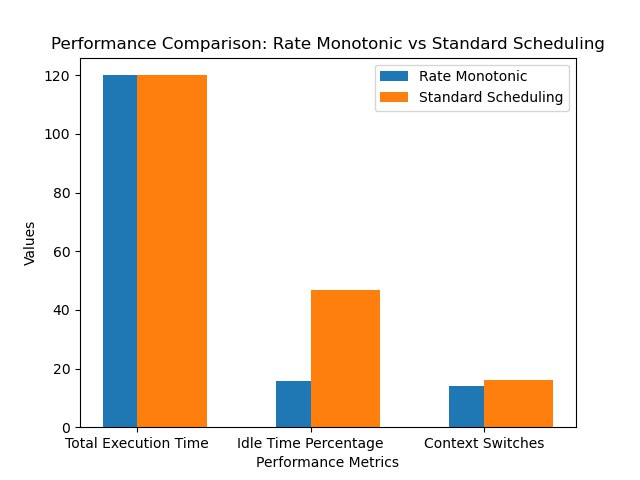
\includegraphics[width=1\linewidth]{img/performance.jpg}
    \caption{Performance Evaluation Comparison (RM Scheduling and Default FreeRTOS Scheduling Algorithm)}
    \label{fig:performance}
\end{figure}

The image shows:
\begin{itemize}
    \item \textbf{Total Execution Time}:
    \begin{itemize}
        \item Both the Rate Monotonic scheduler and the standard FreeRTOS scheduler are executed for 120 seconds.
    \end{itemize}
    \item \textbf{Idle Time Percentage}:
    \begin{itemize}
        \item The standard FreeRTOS scheduler shows a significantly higher idle time percentage compared to the Rate Monotonic scheduler.
        \item This indicates that the RM algorithm is more efficient in utilizing CPU time, reducing the periods when the CPU remains idle.
    \end{itemize}
    \item \textbf{Context Switches}:
    \begin{itemize}
        \item The standard FreeRTOS scheduler has a slightly higher number of context switches compared to the Rate Monotonic scheduler.
        \item Context switches represent the operating system's overhead, so a lower number of context switches in the RM case suggests greater efficiency.
    \end{itemize}
\end{itemize}

\noindent The FreeRTOS scheduler exhibits more idle time because, when tasks have the same priority, FreeRTOS allows multiple tasks to run in parallel (multitasking). This can be both an advantage and a disadvantage when a task is waiting for data from other tasks. Additionally, the context switches are higher in the default FreeRTOS scheduling because multitasking implies that tasks are repeatedly switched after having a common CPU time slice.
\section{Division of Works}
\begin{itemize}
    \item Part 1: Merico Michele, Marino Alberto, Maniero Edoardo, Seidita Nicola
    \item Part 2: Merico Michele, Marino Alberto, Maniero Edoardo, Seidita Nicola
    \item Part 3: Merico Michele, Marino Alberto
    \item Part 4: Maniero Edoardo, Seidita Nicola
\end{itemize}

\end{document} % End of the document
